%! Author = trevo
%! Date = 4/18/2024

% Preamble
\documentclass[12pt]{report}

% Packages
\usepackage{amsmath,geometry,setspace, enumerate,pdfpages,mathrsfs,hyperref,csquotes}
\usepackage[british]{babel}
\usepackage[round]{natbib}
\usepackage{amsfonts}
\usepackage{eufrak}
\bibliographystyle{plainnat}
\doublespacing
\setlength\parindent{24pt}
\newcommand{\Z}{\mathbb{Z}}
\newcommand{\Q}{\mathbb{Q}}
\newcommand{\R}{\mathbb{R}}
\newcommand{\N}{\mathbb{N}}
\newcommand{\U}{\mathfrak{U}}
\begin{document}
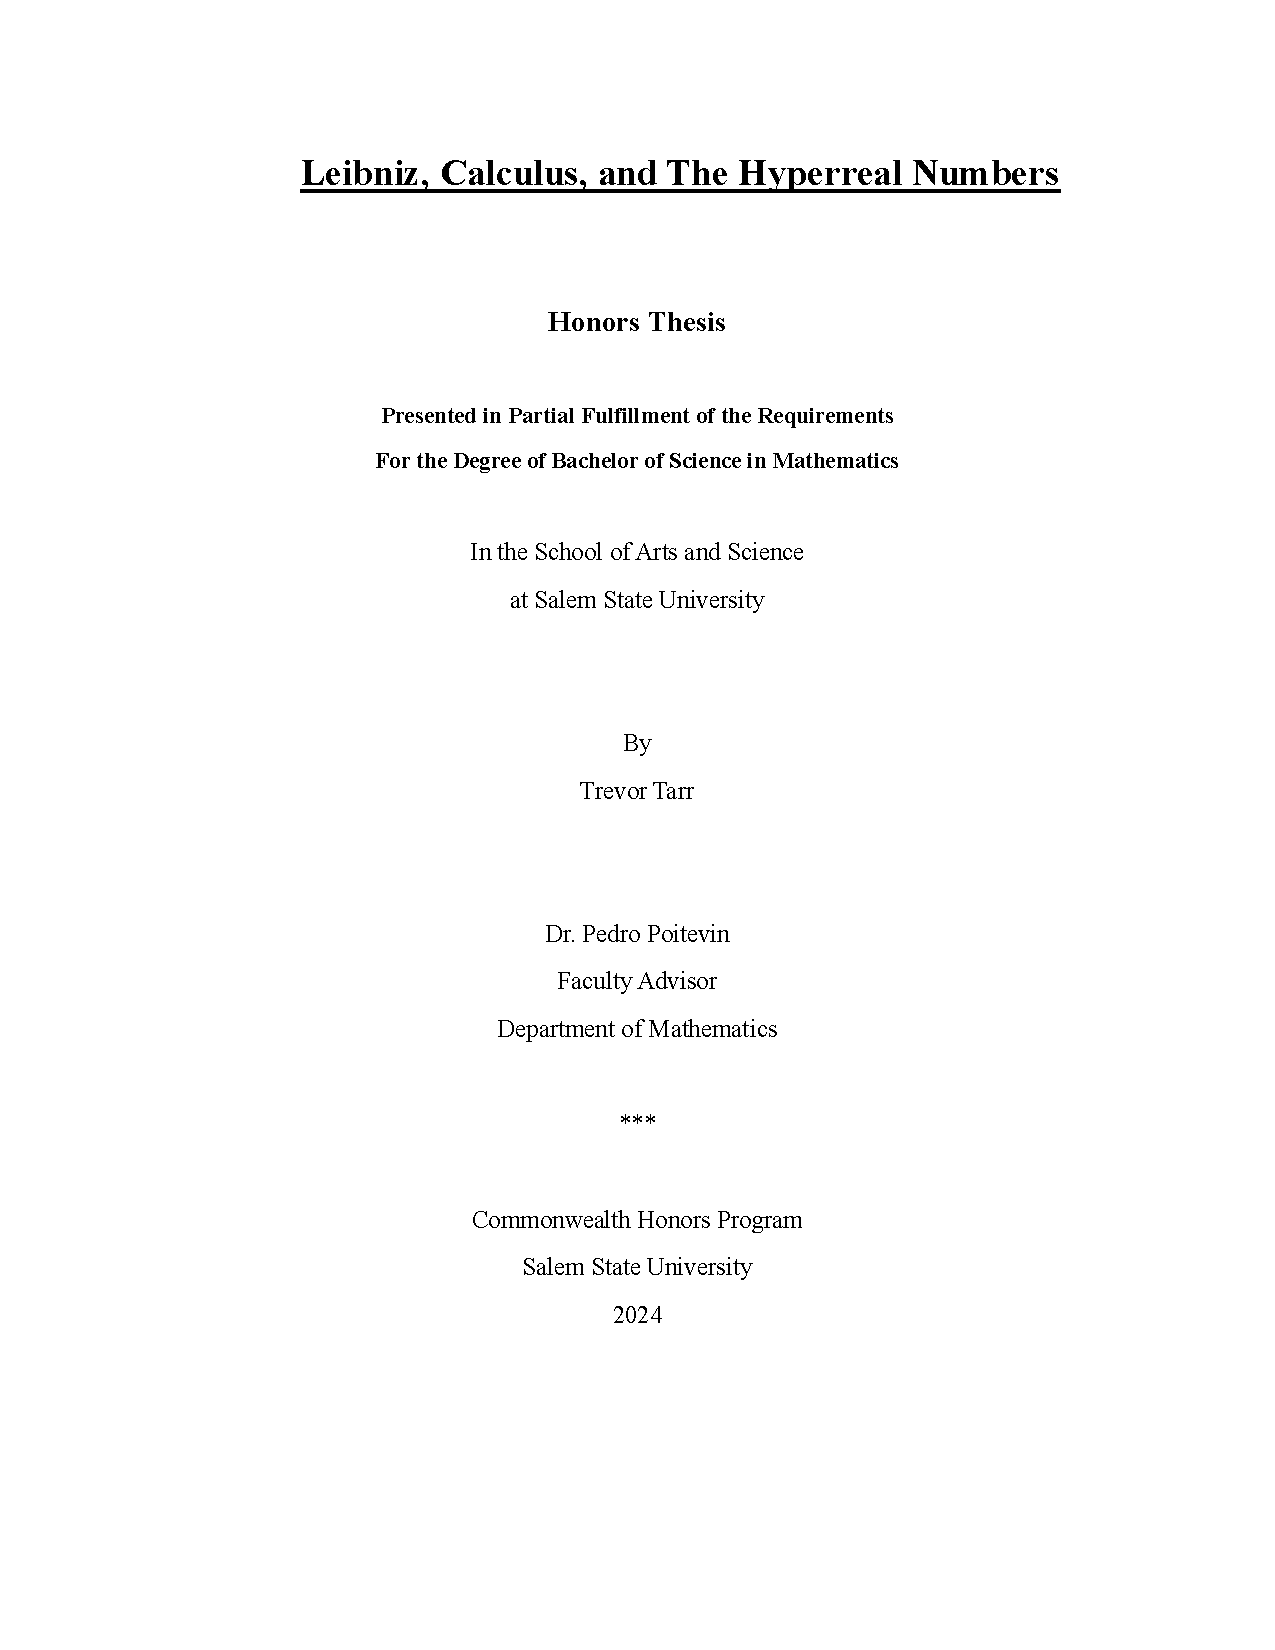
\includepdf[pages=1]{title}
    \newpage
\pagenumbering{gobble}
    \newpage
    \pagenumbering{roman}



\section*{\underline{Abstract}}
Our ideas revolving around Calculus, Philosophy, Law, and Theology are often so clouded that we forget to acknowledge the people behind these ideas.
We are taught these ideas within near hours, days, or as much as months and yet only scratch the surface.
Through this way of thinking, we forget to look at the foundations that took countless years and even lifetimes to construct out of what we believe to be nothingness.
What if I were to say everything mentioned in the first sentence was revolutionized by a German mathematician, philosopher, and logician's name is Gottfried Wilhelm Leibniz(\citauthor{Belaval}).
The first part of this paper will focus on outlining his contributions to the foundations and invention of Calculus, disagreements between him and Newton regarding Calculus, Leibniz's notation for Calculus, and some of his other work in other areas such as law, metaphysics, and much more.
This paper will not cover personal details, including his personal life (birth, death, spouses, etc.) as that does not align with the goals of this paper.\par \\
The second part focuses on Abraham Robertson's construction of the Hyperreal Numbers and their applications proving that Leibniz's intuition of infinitesimals and Calculus correct.
Accurate recognition of one's work is critical in maintaining not only credibility over future pieces of work but also recognizing the accomplishments of one's work.
Understanding Leibniz's work and the instrumental construction of Calculus and infinitesimals allows us to also focus on the foundations of our modern societies and trace where many of our common ideas and innovations stem from.
Ultimately, by the end of this paper, one should have a better understanding of the impact Leibniz, infinitesimals, and the foundational understandings of Calculus.
\newpage
\section*{\textit{Acknowledgements}}
\begin{itshape}
    Firstly, I'd like to thank Gottfried Wilhelm Leibniz himself for his dedication to academia, which expanded our understanding of various structures of society and reason.\newline \newline
    I am extremely grateful for my professor and advisor Dr.Pedro Poitevin, who not only advised me and took time with me to form this work but also educated me in standard and non-standard analysis.\newline\newline
    I would also like to thank Dr.Jeff Theis for working with me to edit and ensure the structure of the work was up to standards.\newline \newline
    Importantly, I want to express my deepest appreciation for the support from my family, including my Mother, Aunt, Grandmother, and others.
    Without them, I would not have had the support and resources to mentally and physically write, study and research this and many other topics simultaneously.
\end{itshape}
\newpage
\pagenumbering{arabic}
\part{Leibniz's Work}
\newpage

\chapter{Infinitesimals}

    \section*{Context}
Leibniz theorized that numbers existed that were infinitely small and/or infinitely great referred to as infinitesimal numbers.
Focused on this idea, Leibniz utilized this idea of infinitesimals to conceptualize the changes in small quantities that led to the idea of the derivative in Calculus (\citauthor{Goldblatt}, 11).
Calculus to Leibniz was the examination and manipulation of infinitesimal values.
While his ideas about infinitesimals were often challenged during his time by many, including Issac Newton, ultimately with the mind of Abraham Robinson in the 1960s, his ideas were ultimately proven to not only exist but also be the fundamental ideas behind calculus, especially when it comes to the derivative and the integral.

\section*{Metaphysical and Theological Perspective}
Leibniz pondered the question on how we live in the most perfect of possible universes.
The idea follows that given some of what he referred to as 'substances' in a non-contradictory combination of existing substances comprise a possible universe in Christian Creationism.
For example, we will use $l, m, n, o, p$ as our substances.
Let's per se we add the following condition onto our substances:
    \begin{enumerate}
        \item Substance $l$ cannot coexist with substance $m$.
        \item Substance $o$ can only coexist with substances $l \ \& \ n$.
    \end{enumerate}
The goal of creation for God, according to Leibniz, is to create a universe with the most substance (most perfect) (\citauthor{Strickland}, 29-31). \\
By this we could get a set containing all the possible.
Some elements can coexist together while some can't.
By creating such a collection of filters, the maximal element of such a filter would be the maximal filter that as such would yield the most perfect universe.
While with four substances it is straightforward, with an unknown amount(most likely infinite) on a grander scale, we can find such a filter used to derive the most perfect universe, which by Leibniz's reasoning on God's perfection in creation, is our universe.
This idea of a maximal element, maximum filter and filters would be where we start to set the scene for the roots of Calculus.

    \section*{The Hyperreal numbers and Continuity}
In 1966, these ideas about maximum filters and infinitesimals are what led mathematician Abraham Robinson to lay out the foundations of what we know today are the Hyperreal number system.
The Hyperreal numbers are an extension of the Real numbers symbolized as infinite sequences of Real numbers (\citauthor{Goldblatt},30-33).
This extension of the real number system allows us to understand continuity and differentiation in calculus the same way as Leibniz had developed roughly 300 years prior.
If two infinitesimals are infinitely close to each other (i.e. $ x \approx c$) then through a function($f$):  $f(x) \approx  f(c)$, (\citauthor{Goldbring}, 81-82).
From here we can say that through the points the function is continuous.
We know that derivative exists for any continuous function in its domain.
Thus, this will bring us into Leibniz's work with derivatives.

    \section*{The Derivative}
To Leibniz, the $dx$ symbol (or with any other letter instead of $x$) symbolized the differential with respect to a variable (or multiple).
Ultimately, the derivative symbolized changes in infinitesimal values based on the slope of the tangent line, as Leibniz has originally proposed (\citauthor{Goldblatt}, 5).
What one is taught is that for finding the derivative is: \[\frac{d}{dx} = \lim_{h \xrightarrow{} \infty} \frac{f(x+h)-f(x)}{h}\] While we are taught that x and h are real numbers, Leibniz proposed that they are what we know as now as hyperreal numbers (as we know of the now) and thus $\frac{dy}{dx}$  is a quotient of infinitesimals describing infinitesimal differences of rate of change.
This idea, while not initially accepted, ultimately was shown to be the foundational idea behind the inner workings of differential calculus.\\ \par
    One way of manipulating derivatives derived by Leibniz is what we know as the Product Rule.
The Product Rule (or Leibniz's Rule) is a method of taking the derivative of two functions that are multiplied. (\citauthor{Leibniz}, 2).
Given two variables $x \ \& \  y$, the derivative of the product is the sum of $x$ multiplied by the derivative of $y$ and $y$ multiplied by the derivative of $x$. As a formula:  $dxy=xdy+ydx$ .

    \section*{The Integral}
Like Riemann Sums, Leibniz idealized that finding the area under any graph starts with finding the area of infinite many polygons under that graph across an infinitesimal interval. 
The $\int$ symbol was Leibniz's notation for integrals derived from the word "Sum" (in Latin: "Summa"). 
This proposition was in conjunction with another credited contributor of what we know as "Integration," Johann Bernoulli. 
Bernoulli originally proposed using a capital "$I$" to denote integration, but to Leibniz's suggestion $\int$ become then deciding symbol as "$I$" closely resembled many other symbols in mathematics (\citauthor{Cajori},412-413).
This would prove to be an insightful suggestion as today many other symbols use Greek and Latin capital lettering and thus would diminish the impact and prevalence of the meaning of integration with a definition like "I". It can also be universally accepted without the knowledge of other languages or confusion with other languages and in programming.  
The use of $dx$ at the end came as a symbol to denote which differential variable was being integrated on.
    
    \chapter{The Rivalry of Leibniz and Newton}
Between 1665 and 1666, Sir Issac Newton first laid out and made known in his work his methods on fluxions.
Newton's ideas revolve around change regarding the passage of time.
His published work known as "\textit{De Analysi}" included his work on these new methods.
Independently, Leibniz developed his ideas in 1675.
His methods focused on the infinitesimal changes of the slope of a general graph (unlike Newton who specifically mentions time as an axis.). While Newton was the first development, Leibniz was the first to publish his work in the mid-1680s through newspaper articles (\citauthor{Bardi}, $v$). \par
While at first acknowledging each other's accomplishments through letter communications, Newton grew ever so paranoid over Leibniz's discoveries.
It had been known that Leibniz had previously looked at Newton's work through a connection and the Royal Society and had taken notes.
Records indicate that these notes we rent used in any manner to claim Newtons work as one's own (\citauthor{Bardi}, 96).
Leibniz proposed an approach to Calculus steered away from Newtons in many aspects.
While Newton mainly stayed on physical-based assumptions and relations to time, Leibniz took the approach to generalize it and focus on the infinitesimals at play.
Newton's paranoia only grew worse as at the same time, Robert Hooke was laying claim to Newton's discoveries laid out in works including "Optiks" (\citauthor{Bardi}, 96).
For another mathematician to have similar ideas at the same exact time and to have met with people.
During both men's remaining time in life, they spent time finding ways to discredit the other.
Even after Leibniz's death, Newton continued to lay claim over all the invention of calculus.\\ \par
While for a long time Newton was the favored, today Leibniz's notations $\int dx$ and $dx$ and his way of thinking using infinitesimals are widely considered standard notations in Calculus (\cite{Goldblatt}, 5).
Leibniz's contributions, though scrutinized during his time, became how we learn and understand Calculus today.
Today, while both men should be recognized and receive equal credit in the invention and development of Calculus, in many instances in education, Leibniz's contributions are pushed aside, with Newton receiving almost full credit even for what is Leibniz's work.
\chapter{More Metaphysics, Law, and Philosophy}
    
\section*{Sin and Evil}
Leibniz on sin and evil stem from his idea mentioned earlier about our universe being the "most perfect" that God could have created.
In that, Leibniz reflects on how since we are in the most perfect would sin must be a part of that most perfectness, according to the criteria placed on by God.
Many argue that "wouldn't a world without evil and sin be the most perfect?", Leibniz touches on that by indicating that if those conditions could exist in such a possible non-contradictory world that we would then be in that by God's perfectness.
Thus, to Leibniz, evil is a part of what he refers to as the most prefect world created.\\ \par
Leibniz lays out three types of sin Metaphysical, Moral, and Physical (\citauthor{Russell}, 197).
To Leibniz, Metaphysical sin is the most important to observe, as at some points he would consider the latter two to be derivatives of metaphysical sin.
Metaphysical sin to Leibniz (in a brief description) is the result of mortal human limitations.
While we are made from a perfect being (God) we still are restricted to our own reason, and thus, while we seek to be perfect, our indeterminate reason leads us to create sin (\citauthor{Strickland}, 206).
We also are limited to knowledge and experience, and as such can only make judgments based on those limited factors. 
Leibniz relates this to Angels as well as being imperfect (such as Lucifer). 
Free to make judgment based on limited knowledge and experience.

\section*{Death Penalty and Torture}
Leibniz on the morality of the death penalty and torture focused on the aspect that we as humans are inevitable determining the weight of a man's life in God's perfect world.
He emphasizes that capital punishment should only be used in such that on a basic level this is a last resort, and the condemned is without any doubt guilty of such a heinous enough crime (\citauthor{Strickland} ,153-154).
One way to decipher this, according to Leibniz, is through a method of torture or including long-term imprisonment.
If the accused demonstrates in some way that there is a possibility of partial innocence, or that capital punishment is too harsh through such treatments (torture or long-term imprisonment), then their execution would in fact bring such guilt on others and as such should not occur (\citauthor{Strickland}, 154).
Through this, we can observe that Leibniz refers to partial innocence rather than full innocence as up to this point it is inferred that some guilt has been proven or confessed to as such methods are not to be used to retrieve new confessions or evidence, only to observe the current state of already known evidence.
While today, we may not implement such methods for traditional trials and discovery methods, his idea about this topic makes us think about the value of a human life when being sentenced.
What we take away from this is the notion of sparingly using capital punishment as a means of justice and when doing so, ensuring that such guilt is proven to the extent that the absence of the person in society is the best course possible.
\newpage
\part{The Hyperreal Numbers}
\newpage
\chapter{Introduction to Construction}

During his lifetime, mathematician Gottfried Leibniz conceptualized values that were infinitely small and/or infinitely great (referred to today as infinitesimal numbers). 
This idea of infinitesimals and changes in such quantities led Leibniz to the conceptualization of the derivative and Integral in Calculus. 
While challenged during his lifetime about the existence of such quantities by many including Issac Newton, ultimately with the help of Abraham Robinson in the 1960s putting together two of Leibniz's greatest ideas (the maximum filter and infinitesimal), his ideas were proven to not only exist but to be the basis of calculus for Integrals and differentials. 
While Leibniz had expressed his ideas on a maximum filter though theological matters such a creationism and the perfect world hypothesis, Abraham Robinson utilized the philosophy of Leibniz's work to create the ultrafilter for the construction of what we know today as the Hyperreal number system (\citeauthor{Goldblatt}, 10-11). 
The Hyperreal numbers are an extension of the Real numbers denoted as infinite sequences of real numbers. 
This extension of the real number system allows many to comprehend continuity and differentiation more simple in calculus the same way as Leibniz thought about them roughly 300 years ago.
Let's begin by going ver a few concepts that will be important to our construction.

\section*{Filters}
A filter is a collection of sets (denoted usually as $\mathbf{F}$) such that it meets the criteria that:
Assuming A and B are non-empty sets:
\begin{itemize}
    \item $\emptyset \not\in \mathbf{F}$
    \item $\text{If }  A \subseteq B \land A  \in \mathbf{F} ,\ \text{then} \ B \in \mathbf{F} $
    \item $\text{If }  A \ \& \ B  \in \mathbf{F} ,\ \text{then}  \ A \cup B \in \mathbf{F} $
\end{itemize}
From this, we can create a superset of all the filters on some set known as the Fr\'echet filter (denoted as $\mathcal{F}$) or the cofinite filter.
One criterion for the Fr\'echet filter is that.
\begin{itemize}
    \item $\text{If } A \in \mathcal{F}, \text{ then } A^c \text{ is finite.}$
\end{itemize}
This is important as we are looking to create infinite sequences, and as such, we want to include any filters that allow for the output of infinite sequences.\\
We will also define the set $J$ with the criterion that:
\begin{itemize}
    \item $\forall B \in J, \mathcal{F} \subseteq B$
\end{itemize}
While right now this set J is not too important, it will come into play for our construction of the Ultrafilter for the Hyperreal numbers.


\section*{UltraFilter}
An ultrafilter ($\mathfrak{U}$ ) is a maximal filter which follows the criterion (along with previous criterions) that:
\begin{itemize}
    \item $\forall A \subseteq J , A \in $\mathfrak{U}$ \lor A^c \in $\mathfrak{U}$ $
\end{itemize}
This criterion follows Leibniz's metaphor using the perfect world.
If we were to have both A and its complement, then any contradictions would exist alongside Leibniz's analogy of perfectness, thus leading to imperfections.
This can lead to sets in the same matter that it will prevent a sufficient maximal element from being achieved.
This leads into the construction of amn ultrapower through Zorn's Lemma.
\subsection*{Zorn's Lemma}
Zorn's Lemma states that all partially ordered sets in a chain that contain an upper bound contain a maximal element.
Partially ordered regarding sets comes down to meeting three criteria:\\
Let $x,y,z \in A$.
\begin{itemize}
    \item Reflexive: If $x \in A$, then $x\leq x$.
    \item Anti-Symmetry If $x,y \in A$, $x\leq$ and $y\leqx$, then $x=y$.
    \item Transitive: If $x \leq y$, and $y \leq z$, then $x \leq z$.
\end{itemize}
The chain refers to the inclusion principle as our partial ordering scheme.
$A_i \subset B$ ,then $A_1\subseteq A_2\subseteq A_3\subseteq\ldots$ is a chain.
Our upper bound is then $\bigcup_{i=1}^{\infty}A_i$.
With these criteria met, there must exist some maximal element according to Zorn's Lemma.

\chapter{Construction}
We know that, $\R^2 $ symbolizes the ordered pair for $x, y \in \R: (x, y)$ and so on for $\R^n$ for $n \in \N$.
What if we raise the set of natural numbers ($\N$) to$ \R$ such as $\R^{\N}$.
This would result in an N-tuple or an infinite sequence of real numbers.
This does, however, raise a few issues.
One issue is that one sequence could be $(5,4,3,2,1,0,-1,\ldots)$ and another be $(\phi,3,\phi, 2,1,0,-1,\ldots)$ are these different notations for the same value?
Another issue is that we do not know if we have everything we can.
Could we saturate more values within this system?
To solve these issues, we can construct an ultrafilter on the natural numbers.\par

Using understanding of filters, we can construct filters on $\N$ containing subsets of the power set of $\N$.
We then create a Fr\'echet filter ($\mathcal{F}$) on $\N$ such that any infinite subset of the power set is in $\mathcal{F}$ and not its complement (which would be finite).
Adding in all subsets (we will denote as $B$) into a common superset ($J$) described as:\[J=\{\forall B\ \in J\ |\ \mathcal{F}\ \subseteq B\ \ \}.\]
Now utilizing Zorn's Lemma, for all $B$ in $J$ we know that through the partially ordering through an inclusion principle chain $B_1\subseteq B_2\subseteq B_3\subseteq\ldots\subseteq B_i\in J $ and its upper bound is then $\bigcup_{i=1}^{\infty}A_i$ then there is some maximal element which is our Ultrafilter ($\U$) on $\N$.
Thus, we have $\R^{\mathfrak{U}} $.


\chapter{ Describing the Hyperreals}
We still have the issue that do we know if $(5,4,3,2,1,0,-1,\ldots)$ and $(\phi,3,\phi, 2,1,0,-1,\ldots)$ are different notations for the same value?
Just as in the real numbers, we can create equivalence classes for these Hyperreal numbers.
We define our equivalence classes such that (\citauthor{Goldbring}, 14 ):
\[\mathrm{Let\ a,b\ \in \R^{\U}}.\ If\ (a)\ \sim_{\U}\ (b)\ then\ the\ set\ \ \{\ n\ \in \N|\ a_{n}\ =\ b_{n}\ \ \}\ \in \U \}\]
In words, this relationship is defined as if the set of coordinates that are the same for $a$ and $b$ is in the Ultrafilter then $a$ and $b$ are equivalent.
This makes sense as these sets would be infinite, and our ultrafilter contains infinite sets of natural numbers and thus infinite sets of similar coordinates.
Note that all real numbers expressed as Hyperreal are infinite sequences of that real number.
For example, the Hyperreal representation of 3 is $(3,3,3,3,3, 3, \ldots)$ and $\pi$ is $(\pi, \pi, \pi,\pi, \pi, \pi, \ldots)$.
\section*{Basic Ordering}
Regarding ordering, we can say that given two distinct Hyperreal equivalence classes $  [[a]]_{\U}, [[b]]_{\U} \ \& \ [[a]]_{\U}\not= [[b]]_{\U} $ that: $ [[a]]_{\U}< [[b]]_{\U} \text{ if }\{a_n < b_n | n \in \N \} \in \U $ if the set of coordinates on $[[a]]_{\U}$ and $[[b]]_{\U}$ that $a_n < b_n$ with $n \in \N $ is in the ultrafilter.
We know this by properties of real numbers.
We know that for real numbers, ordering properties hold (full explanation is beyond the scope of this paper) and thus for each real number coordinate $a_n, b_n$, we can construct a set containing the coordinates of every instance where $a_n < b_n | n \in \N$.
If the set is infite, then by our construction, the set is in the ultrafilter.
Thus, we've established an ordering relationship between $[[a]]_{\U}$ and $[[b]]_{\U}$ and consequently on the Hyperreal numbers.

\section*{Field}
While we have basic ordering and equivalence classes for Hyperreal, we want to prove that they form a field.
To do this, we will prove:
\begin{enumerate}
    \item They are a group under addition.
    \item The non-zero equivalence classes form a group under multiplication.
    \item The distributive property holds.
    \item The negative of a Hyperreal is less than its positive.
\end{enumerate}
For the next sections we will define $x,y,z$ to be Hyperreal numbers such that: x =[[x]]_{\U}, y= [[y]]_{\U}, z=[[z]]_{\U}.
\subsection*{Group Properties}
We will start by proving that it is a group under addition.
To prove that the Hyperreals are a group, we must prove that under the binary operation of addition that the Hyperreal are Closed, Associativity, the Identity exists, and the Inverses exist.
Since the Hyperreal numbers are an extension of the real numbers, properties of the real numbers will assist us in proving these.
\begin{enumerate}
    \item[Closure:]Let $x$ and $y$ be in $\R^\U $.
    Since each coordinate of $x$ and $y$ are real numbers, addition of $x$ and $y $ is the addition of each corresponding coordinate: $x+y$ = $(x_1 + y_1, x_2+y_2,\ldots)$.
    Since the real numbers are closed under addition, each coordinate will be a real number, thus $x+y$ is in $\R^\U$.
    \item[Associvity:]Since each coordinate of $x$,$y$ and $z$ are real numbers, associativity of $x$ and $y $ is the addition of each corresponding coordinate: $(x+y)+z = ((x_1 + y_1)+z_1, (x_2+y_2)+z_2,\ldots) =x+(y+z) = (x_1 + (y_1+z_1), x_2+(y_2+z_2),\ldots)$.
    Thus $(x+y)+z= x+(y+z)$.
    \item[Idenity:]We know for standard addition in the non-zero real numbers, the identity is $[[0]]_{\U}$.
    The Hyperreal representation of $[[0]]$ is $(0, 0, 0,\ldots)$.
    \item[Inverses:]There exist Hyperreal numbers $x, x'$ such that $x+x' = e $ where $e$ is our identity element.
    We know our identity element to be $(0, 0, 0, \ldots)$.
    Subtracting $x$ on each side, we get $x' = (0, 0, 0,\ldots) - x = -x or (-x_1, -x_2, -x_3,\ldots)$. We apply the same logic for $x' +x = e $ as we cannot assume communitivity.
    This works out to be the same.
\end{enumerate}
Thus, The Hyperreal Numbers are a group under addition.
\newline \par We will state just for it to be noted that since addition in the reals is also commutative so is true for hyper real numbers as well.
This logic will fall over into multiplication as well.
Going into multiplication for non-Zero Hyperreal numbers. \newline \par


We will now prove that for the non-zero Hyperreals under multiplication are a group.
\begin{enumerate}
    \item[Closure:]Let $x$ and $y$ be in $\R^{\U}$.
    Since each coordinate of $x$ and $y$ are real numbers, multiplication of $x$ and $y$ is the multiplication of each corresponding coordinate: $xy = (x_1 y_1, x_2 y_2,\ldots)$ .
    Since the real numbers are closed under multiplication, each coordinate will be a real number thus $xy$ is in $\R^\U$.
    \item[Associvity:] Since each coordinate of $x$,$y$ and $z$ are real numbers, associativity of $x$ and $y $ is the addition of each corresponding coordinate: $(xy)z = ((x_1 y_1)z_1, (x_2 y_2)z_2,\ldots) =x(yz) = (x_1  (y_1 z_1), x_2(y_2 z_2),\ldots)$.Thus $(xy)z= x(yz)$.
    \item[Idenity:]We know for standard addition in the non-zero real numbers, the identity is $[[1]]_{\U}$.
    The Hyperreal representation of $[[1]]$ is $(1, 1, 1,\ldots)$.
    \item[Inverses:]There exist Hyperreal numbers $x, x'$ such that $xx' = e $ where $e$ is our identity element.
    We know our identity element to be $(1, 1, 1, \ldots)$.
    multiply $\frac{1}{x}$ on each side, we get $x' = \frac{(1, 1, 1,\ldots)}{x} = \frac{1}{x} or (\frac{1}{x_1}, \frac{1}{x_2}, \frac{1}{x_3},\ldots)$We then apply the same logic for $a^{-1} a =1$ as we cannot assume commutativity.
    This turns out to be also true.
    This then also means that for $\frac{1}{a_n}$ the set ${n \in \N| a_n not 0 } \in \U$.
    Thus, our inverses exist.
\end{enumerate}
\subsection*{Connective Tissue Properties}
Finally, for a field, we will prove the connectivity tissue under addition and multiplication holds for the Hyperreal numbers.
\newline \par
For the distributive property, since the hyperreal numbers are an extension of the real numbers, the distributive property holds the same in the Hyperreal as in the reals.
We use the same idea that it holds for every real number coordinate that make up the Hyperreal.
This translates to:\newline Since for every coordinate $x_n(y_n+z_n) = x_n y_n + x_n z_n$ then $x(y+z)= xy+xz$.\newline


We next must prove high level ordering properties for the Hyperreal numbers. \newline
We want to show that if $x<y$ and $z>0$ then $xz<yz$. \\
Let $A$ be the set of coordinates of $a<b$ using the definition of ordering created in the section of the same name.
Let $B$ be the set of coordinates of $c$ such that for every coordinate $z_n > 0$.
Multiplying each side of $x<y$ by $z$ we get $xz<yz$.
This relationship is equivalent to finding the intersection of A and B.
We know by filter properties the intersection is $\U$.
Thus, by basic ordering properties (see section on basic ordering principles above) $xz<yz$.
This same logic will follow for showing that $x+z < y+z$.

\newline \par
Finally, we will prove that $-x <x $for non-zero Hyperreal numbers.
Note that $x$ is positive.
We know that the negative of a Hyperreal is represented by the infinite sequence of the negative of each coordinate: $-(x_1, x_2,x_3,\ldots) = (-x_1,- x_2,-x_3,\ldots)$ .
We know that since each coordinate is a real number, properties of real numbers hold for each coordinate.
We know that given a positive real numbers $r$, that $-r< r$ for all non-zero real numbers.
Since for every real number coordinate $-x_n <x_n for n \in \N $ then by our definition of ordering, the set ${n \in \N| -x_n < x_n } \in \U$.
Thus, $-x <x $.

\\ \newline
Thus, we have a non-standard field $\R^{\U}$.\\
Q.E.D.


\chapter*{Applications}
We will now dive into two areas of application for Hyperreal numbers.
Note that this is not teh only applicatiosn as Hyperreal numbers are one of the main concepts of non-standard analysis.
\section*{Continuity}
Using the Hyperreal, we can show continuity in a more streamlined manner than with standard analysis.
Typically, one shows continuity by first showing that for every point in the domain that the limit between two points is below some small epsilon value and then one can say that those two points through a function are infinitely close.
With the Hyperreal numbers, we can say that two Hyperreal numbers are infinitely close to each other (that is $|x-y|< \epsilon$) then through the function they continue to be infinitely close (that is |$f(x)-f(y)|<\varphi$) (\citauthor{Goldbring},25) thus showing continuity.
We know as well that if a function is continuous, it is all differentiable (a derivative exists for the function).
This idea is what Leibniz used to formulate his ideas about Calculus and differentials and touched upon in his Theory of Optimism.

\section*{Complex Hyperreals}
As with real numbers, there exists such number aptly named the ‘Hypercomplex numbers’ comprised of both a Hyperreal and complex aspect.
If $ a,b$ are Hyperreal numbers ($[[a]]_{\U} \  \& \  [[b]]_{\U}$) then a Hypercomplex number would be in the form $a+bi$.
The $bi $ component can also be represented as $(ib_1, ib_2,\ldots)$.
The construction of such a system is beyond the scope of this exploration but still is possible.


\chapter*{\underline{Conclusion}}
Gottfried Wilhelm Leibniz was a logician, philosopher, and innovator that ultimately changed the way we interact and think about various topics such as how we perceive changes in rates and infinitesimals to law and ethics, to even Theology.
While some of his views (mainly calculus) came at time in parallel with others who lay to claim on the matter and at the time used their influence to outweigh Leibniz, today we realize the true impact Leibniz had on our world.
I have also gained both a better understanding of calculus and constructions of number systems through abstract thinking.
The application of philosophy onto mathematics through this research has shown to me the abstract thinking aspects of developing new mathematically sound theorems and proofs.
I now also have a better understanding of how calculus works and who we do what we do in calculus.
From differentials and infinitesimals to integration and the hyperfinite numbers (a subset of the hyperreal numbers as the Natural numbers are to the reals).
\par


In future with regard to research into Leibniz, I would much like to investigate more of his work as a philosopher.
His works regarding Law and Ethics stick out to me the most as his ideas on Metaphysics and Theology establish criteria and reason on how to pass judgment and complex structures of human ethics. \par
Leibniz's impact on today rivals many others in history as his research expanded into numerous disciplines and even created bridges between such disciplines such as mathematics, metaphysics, and theology.
His ingenuity has affected billions of people over the course of multiple generations, and to this day we utilize many of his ideas such as calculus, ethics around capital punishment, and intuitions and understanding of theology.\par \\

With regard to the infinitesimals and hyprreal numbers, I would like to mainly take this research in two directions.
First, I would like to research new ways to apply hyperreal numbers into mathematics.
Specifically, sociology and human sciences as those areas interest me most.
Secondly, I would want to continue into non-standard analysis and research this area of mathematics more in-depth.
While the hyperreal numbers were just an introduction, I would like to delve deeper into topics including probability theory, applied mathematics (with infinitesimals), and differential equations.
Overall, my understanding of mathematics, historical mathematics, Leibniz and complex structures has grown throughout my research.
\newpage
    \bibliography{resources}
\end{document}